\documentclass[]{scrartcl}

\usepackage {listings}
\usepackage[ngerman]{babel}
\usepackage[utf8]{inputenc}
\usepackage{graphicx}
\usepackage{xcolor}
\usepackage{hyperref}

\setlength{\parindent}{0em}

%opening
\title{Warenlagerung eines Kaufhauses}
\subtitle{Evolutionäre Algorithmen - SL3 - Soft Computing - SS17}
\author{Benedikt Straube}

\begin{document}

\maketitle

\newpage

\section{Installation}
Zur lokalen Ausführung der Applikation ist eine NodeJs Installation notwendig. Diese sollte mindestens in Version 6.11.0 (\url{https://nodejs.org/}) zur Verfügung stehen.

Im nächsten Schritt sollten innerhalb des Projektverzeichnisses die notwendigen Pakete für eine lokale Ausführung installiert werden. Dies ist möglich via 
\begin{lstlisting}[backgroundcolor=\color{lightgray}]
npm install
\end{lstlisting}

Nachdem alle notwendigen Pakete installiert wurden, kann ein lokaler Server mittels
\begin{lstlisting}[backgroundcolor=\color{lightgray}]
npm start
\end{lstlisting}
gestartet werden.

Danach ist die Applikation im Browser über \url{http:localhost:4200} zu erreichen.


\section{Ausführung}
\label{ausfuehrung}
Die Applikation kann über die beschriebe Installation lokal gestartet und über den Browser bedient werden. Weiterhin wird der compilierte Code zusätzlich über GitHub-Pages gehostet. Dadurch ist die Applikation auch unter der URL \url{https://benediktst.github.io/Soft-Computing-VAWI} zu erreichen.

Vorsicht: Hier existiert zum aktuellen Zeitpunkt noch ein Bug des Routings, was bei dem Refresh der Applikation zu einer 404-Seite führt. Die Applikation kann immer wieder über die Angegebene URL erreicht werden.

\begin{figure}[htbp]
	\centering
	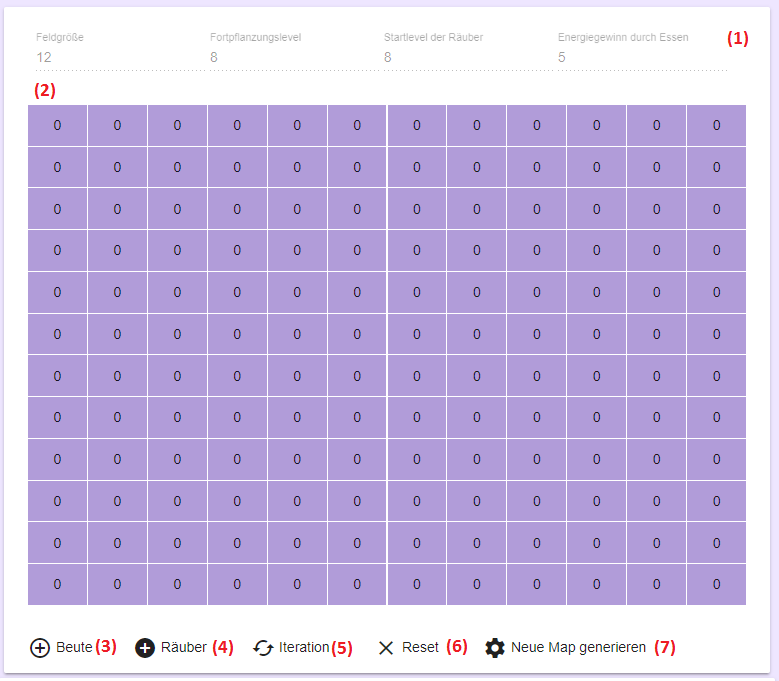
\includegraphics[width=0.7\textwidth]{res/interface.png}
	\caption{Aktionsmöglichkeiten der Anwendung}
	\label{img:interface}
\end{figure}

Um die Implementierung der SL-3 zu erreichen muss innerhalb der Kopfzeile ganz rechts das Menü geöffnet und die Option SL-3 ausgewählt werden. In der Anwendung (siehe Abbildung \ref{img:interface}) können an erster Stelle (1) die Ausgangsdaten eingesehen werden. Diese sind für diese Implementierung statisch im Code hinterlegt und sind hier lediglich informativ. Bei den Aktionen steht zuerst die Generierung der Kinder (2) zur Verfügung. Dies geschieht nach einer (10/2,15)- Evolutionsstrategie, wodurch basierend auf den zufällig generierten Eltern 15 neue Vektoren entstehen. Dabei werden diese durch Mittelwertbildung erzeugt. Die Bewertung (3) fügt eine Bewertung zu jedem Vektor hinzu. Die Eltern erhalten ebenfalls eine Bewertung, auch wenn sie für nie nachfolgende Generation nicht weiter betrachtet werden. Bei der Mutation (4) wird eine statische Standardabweichung auf alle Bestandteile der Vektoren angewendet, um die notwendige Varianz zu erhalten. Die dadurch entstehenden Vektoren werden dann als neue Elterngeneration verwendet. Bei der 50-fachen Iteration (5) werden die vorherigen drei Schritte entsprechend häufig wiederholt. Im unteren Bereich (6) werden die Eltern und Kinder mit Bewertung dargestellt.

\section{Aufbau der Applikation}
\label{aufbau}
Das Framework zur Implementierung ist Angular. Es nimmt keine bedeutenden Eingriffe in die Implementierung der Logik, sondern übernimmt hauptsächlich die Darstellung innerhalb des Browsers.


Die Implementierung erfolgt innerhalb nachfolgender Orderstruktur:
\begin{lstlisting}[backgroundcolor=\color{lightgray}]
src
|- app
   |- ea
\end{lstlisting}
Außenstehende Komponenten sind zur Navigation und Verwaltung notwendig.

Innerhalb des EA-Ordners befinden sich folgende Dateien:
\begin{itemize}
\item ea.component.css (Styling der Komponente)
\item ea.component.html (Strukturierung der Komponente)
\item ea.component.ts (Logik der Komponente)
\end{itemize}

Im util-Ordner stehen noch weitere Klassen zur Verfügung, auf welche im Folgenden genauer eingegangen werden soll.
\begin{itemize}
	\item product.model.ts (Modell eines Produktes)
	\item vektoren.model.ts (Abbilden und Bewerten eines Vektors)
\end{itemize}

Die \textit{Produkt}-Klasse enthält alle für die Produkte notwendigen Informationen. Dies beinhaltet den Namen, die anteilige Lagergröße, die Lieferdauer, der Verbrauch und der Lagerbestand. Die Produkte an sich benötigen keine weitere Logik.

Die \textit{Vektoren}-Klasse besitzt zwei Arrays, welche für die reelle Codierung relevant sind: \textit{minimalStock} und \textit{buyAmount}. Innerhalb von minimalStock wird für jedes Produkt festgehalten, ab wann nachgekauft werden sollte, buyAmount enthält entsprechend die nachzukaufende Menge. Diese werden auch innerhalb der \textit{toString}-Methode zur Visualisierung verwendet. Hier werden sie allerdings jeweils Pro Produkt dargestellt, also [minimalStock(Prod A), buyAmount(Prod A)], ... (siehe Abbildung \ref{img:vektoren}). Ergänzt wird diese Darstellung durch die Bewertung der einzelnen Vektoren und eine durchschnittliche Fitness über die gesamte Generation.

\begin{figure}[htbp]
	\centering
	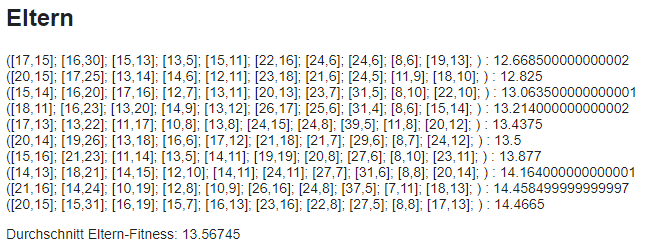
\includegraphics[width=0.7\textwidth]{res/vektoren.png}
	\caption{Darstellung der Elternvektoren}
	\label{img:vektoren}
\end{figure}



\section{Ergebnisse}
\label{ergebnisse}
Als erstes muss angemerkt werden, dass bereits während der Entwicklung deutlich wurde, dass die Ermittlung des gesamten Lagerbestandes ein Problem darstellt. Die Information ist für die Regeln notwendig und die ersten Ansätze zur Ermittlung mit den logischen Operatoren UND und ODER führten zu ausschließlich Extremwerten. Nachdem so keine gleichmäßige Verteilung erreicht werden konnte, wurde die Berechnung auf eine Durchschnittsbildung innerhalb der einzelnen Menge angepasst. Die Ergebnisse  scheinen so besser verteilt und passen logisch trotzdem zu den Werten des Lagerbestands.
\\

Interessant ist die asymmetrische Verteilung der Teilmengen sowohl bei der Nachfrage als auch beim Lagerbestand. Dies führt dazu, dass die Empfehlungen sich nicht überwiegend im Bereich ''mittel'' zu 100\% bewegen, sondern tatsächlich eine ausreichende Varianz aufweisen. Gerade die "niedrig" Teilmengen zu beiden Sets nehmen bei einer zufälligen Verteilung zwar etwas weniger Platz ein, jedoch agieren die Regeln so, dass sowohl eine geringe Nachfrage als auch ein geringer Bestand im Lager starken Einfluss auf die Kaufentscheidung nehmen.
\\

Auffällig ist ebenfalls, dass bereits bei drei Teilmengen eine relativ hohe Anzahl an Regeln notwendig war, um sinnvolle Empfehlungen zu geben und dennoch weiteres Verbesserungspotenzial besteht. Daraus lässt sich ableiten, dass bei einer detaillierteren Unterteilung der Gesamtmenge in eine größere Zahl an Teilmengen eine stets noch höhere Anzahl an Regeln notwendig ist, um beständig sinnvolle Entscheidungen zu generieren. Gerade bei einem vollständig automatisierten System, welches in einem solchen Szenario automatisch die Bestellungen vornehmen müsste, wäre eine aufwändige manuelle Erstellung und Qualitätssicherung der Regelbasis notwendig. Es ist also definitiv bemerkbar, dass die Komplexität eines solchen Expertensystems nicht in der Umsetzung oder Konzeption der Fuzzy-Logik, sondern in der Regelbasis liegt. 

\end{document}
